\documentclass{article}
\usepackage[utf8]{inputenc}
\usepackage{geometry}
\usepackage{amsmath}
\usepackage{amsfonts}
\usepackage{graphicx}


\geometry{
 a4paper,
 total={170mm,257mm},
 left=15mm,
 right=15mm,
 top=10mm,
 }

\title{TP-P7}

\begin{document}

\begin{center}
\hrule
	\vspace{.4cm}
	{\textbf { \large TP P3}}
\end{center}

{\textbf{Nom:}\ Arnaud Lelièvre et Calypso Derven \hspace{\fill} \vspace{0.5cm}}
{\textbf{Date: samedi 29 Janvier}\  \hspace{\fill} \vspace{0.5cm}}
{\textbf{chapitre : P7}\ \hspace{\fill}}
\hrule
\date{}

\vspace{1cm}

\begin{center}
\textbf { \large Etude d'un condensateur}
\end{center} \vspace{0.2cm}

\section{Comportement capacitif}
\subsection{}
En fermant l'interrupteur, $D_1$ et $D_3$ s'allument, puis $D_1$ s'éteint progressivement.
\\

\subsection{}
En ouvrant l'interrupteur, $D_2$ s'allume, $D_3$ s'éteint, et $D_2$ s'éteint progressivement. \\

\subsection{}
Lorsque l'on ferme l'interrupteur, $D_3$ s'allume car elle est en circuit fermé. quand on ouvre l'interrupteur, le circuit de $D_3$ est ouvert donc $D_3$ s'éteint. \\
Lorsque l'on ferme l'interrupteur, le condensateur ce charge et agit comme la terre, donc le courrant passe jusqu'à ce que condensateur soit complètement chargé, donc pendant ce temps là $D_1$ s'allume, et s'éteint progressivement tel que quand le condensateur est chargé, $D_1$ soit complétement éteint. \\
Si le condensateur est chargé, alors quand on ouvre l'interrupteur, le condensateur se décharge, et agit comme un générateur, et donc $D_2$ s'allume lorsque le condensateur se décharge. \\

\section{Détermination du temps caractéristique et de la capacité d'un condensateur}

\large{\textbf{a)}} \\
En utilisant la methode des $63\%$, on peut déterminer $\tau$. Il est dit que $\tau$ est le temps ou $u_c(t)$ atteint $63\%$ de sa tension maximal, soit $E$. \\
Donc, on a $u_c(\tau) = 0.63 \cdot E \leftrightarrow u_c(\tau) = 0.63 \cdot 12 = 7.56V$ \\ \\
Par lecture graphique on repère l'abscisse dont le point dont l'ordonnée est $7.56V$, et on obtient $\tau = 0.05433 s$. Afin d'obtenir $C$, on a la relation $\tau = RC \leftrightarrow C = \frac{\tau}{R}$, or on a $R = 5k\Omega$. Donc, on a $C = \frac{0.05433}{5 \cdot 10^3} = 1.09 \cdot 10^{-5}F$ \\ \\
\large{\textbf{b)}} \\
Avec Atelier scientifique, on trace la tangeante à $u_c(t)$ à $t = 0$, et on obtient la tangeante à l'origine, qui coupe l'asymptote horizontale d'équation $y = E$ en $\tau$, par lecture graphique, on a l'abscisse du point d'intersection des tangeantes qui est $t = 0.05276 s$, donc, on a $\tau = 0.05276 s$, et donc, on a $C = \frac{\tau}{R} = \frac{0.05276}{5 \cdot 10^3} = 1.0552 \cdot 10^{-5} F$ \\ \\
\large{\textbf{c)}} \\
On a \\

$ln({\frac{E - u_c(t)}{E}})$ \\
$= ln({\frac{E - E(1-e^{-\frac{t}{\tau}})}{E}})$ \\
$= ln({1 - (1-e^{-\frac{t}{\tau}}}))$ \\
$= ln({1 - 1 + e^{-\frac{t}{\tau}}}))$ \\
$= ln({e^{-\frac{t}''\tau}}))$ \\
$= -\frac{t}{\tau}$ \\
$= t ({-\frac{1}{\tau}})$ \\
\\

En tracant $ln({\frac{E - u_c(t)}{E}})$, on obtient donc une droite de coefficient directeur $({-\frac{1}{\tau}})$, or la pente de la courbe est de $17.1 \leftrightarrow \tau = \frac{1}{17.1} = 0.05848 s$. \\

Donc $C = \frac{\tau}{R} = \frac{0.05848}{5 \cdot 10^3} = 1.17 \cdot 10^{-5} F$ \\ \\
\large{\textbf{d)}} \\
Par lecture graphique, on a un point de la courbe de coordonnées $(0.05438, 7.54)$ \\

Or, on a $u_c(t) = E(1 - e^{-\frac{t}{\tau}})$ \\

$\leftrightarrow 1 - e^{-\frac{t}{\tau}} = \frac{u_c}{E}$ \\
$\leftrightarrow e^{-\frac{t}{\tau}} = 1 - \frac{u_c}{E}$ \\
$\leftrightarrow -\frac{t}{\tau} = ln({1 - \frac{u_c}{E}})$ \\
$\leftrightarrow \tau = -\frac{t}{ln({1 - \frac{u_c}{E}})}$ \\

Avec $(0.05438, 7.54)$, on a \\

$\tau = -\frac{0.05438}{ln({1 - \frac{7.54}{12}})} = 0.0549 s$ \\

Donc $C = \frac{\tau}{R} = \frac{0.05549}{5 \cdot 10^3} = 1.09 \cdot 10^{-5} F$ \\ \\
\large{\textbf{e)}} \\
Les valeurs sont donc cohérentes entre elles, donc toutes ces émthodes permettent de trouver $\tau$ avec précision (avec une incertitude proche de $10\%$).
\begin{center}
    \large{\textbf{graphique représentant les courbes modélisant $u_c(t)$ (bleu), $E(t)$ (rouge), $y = \frac{u_c}{dt}(0) t$ (violet), $ln({\frac{E - u_c(t)}{E}})$ (gris)}} \\
    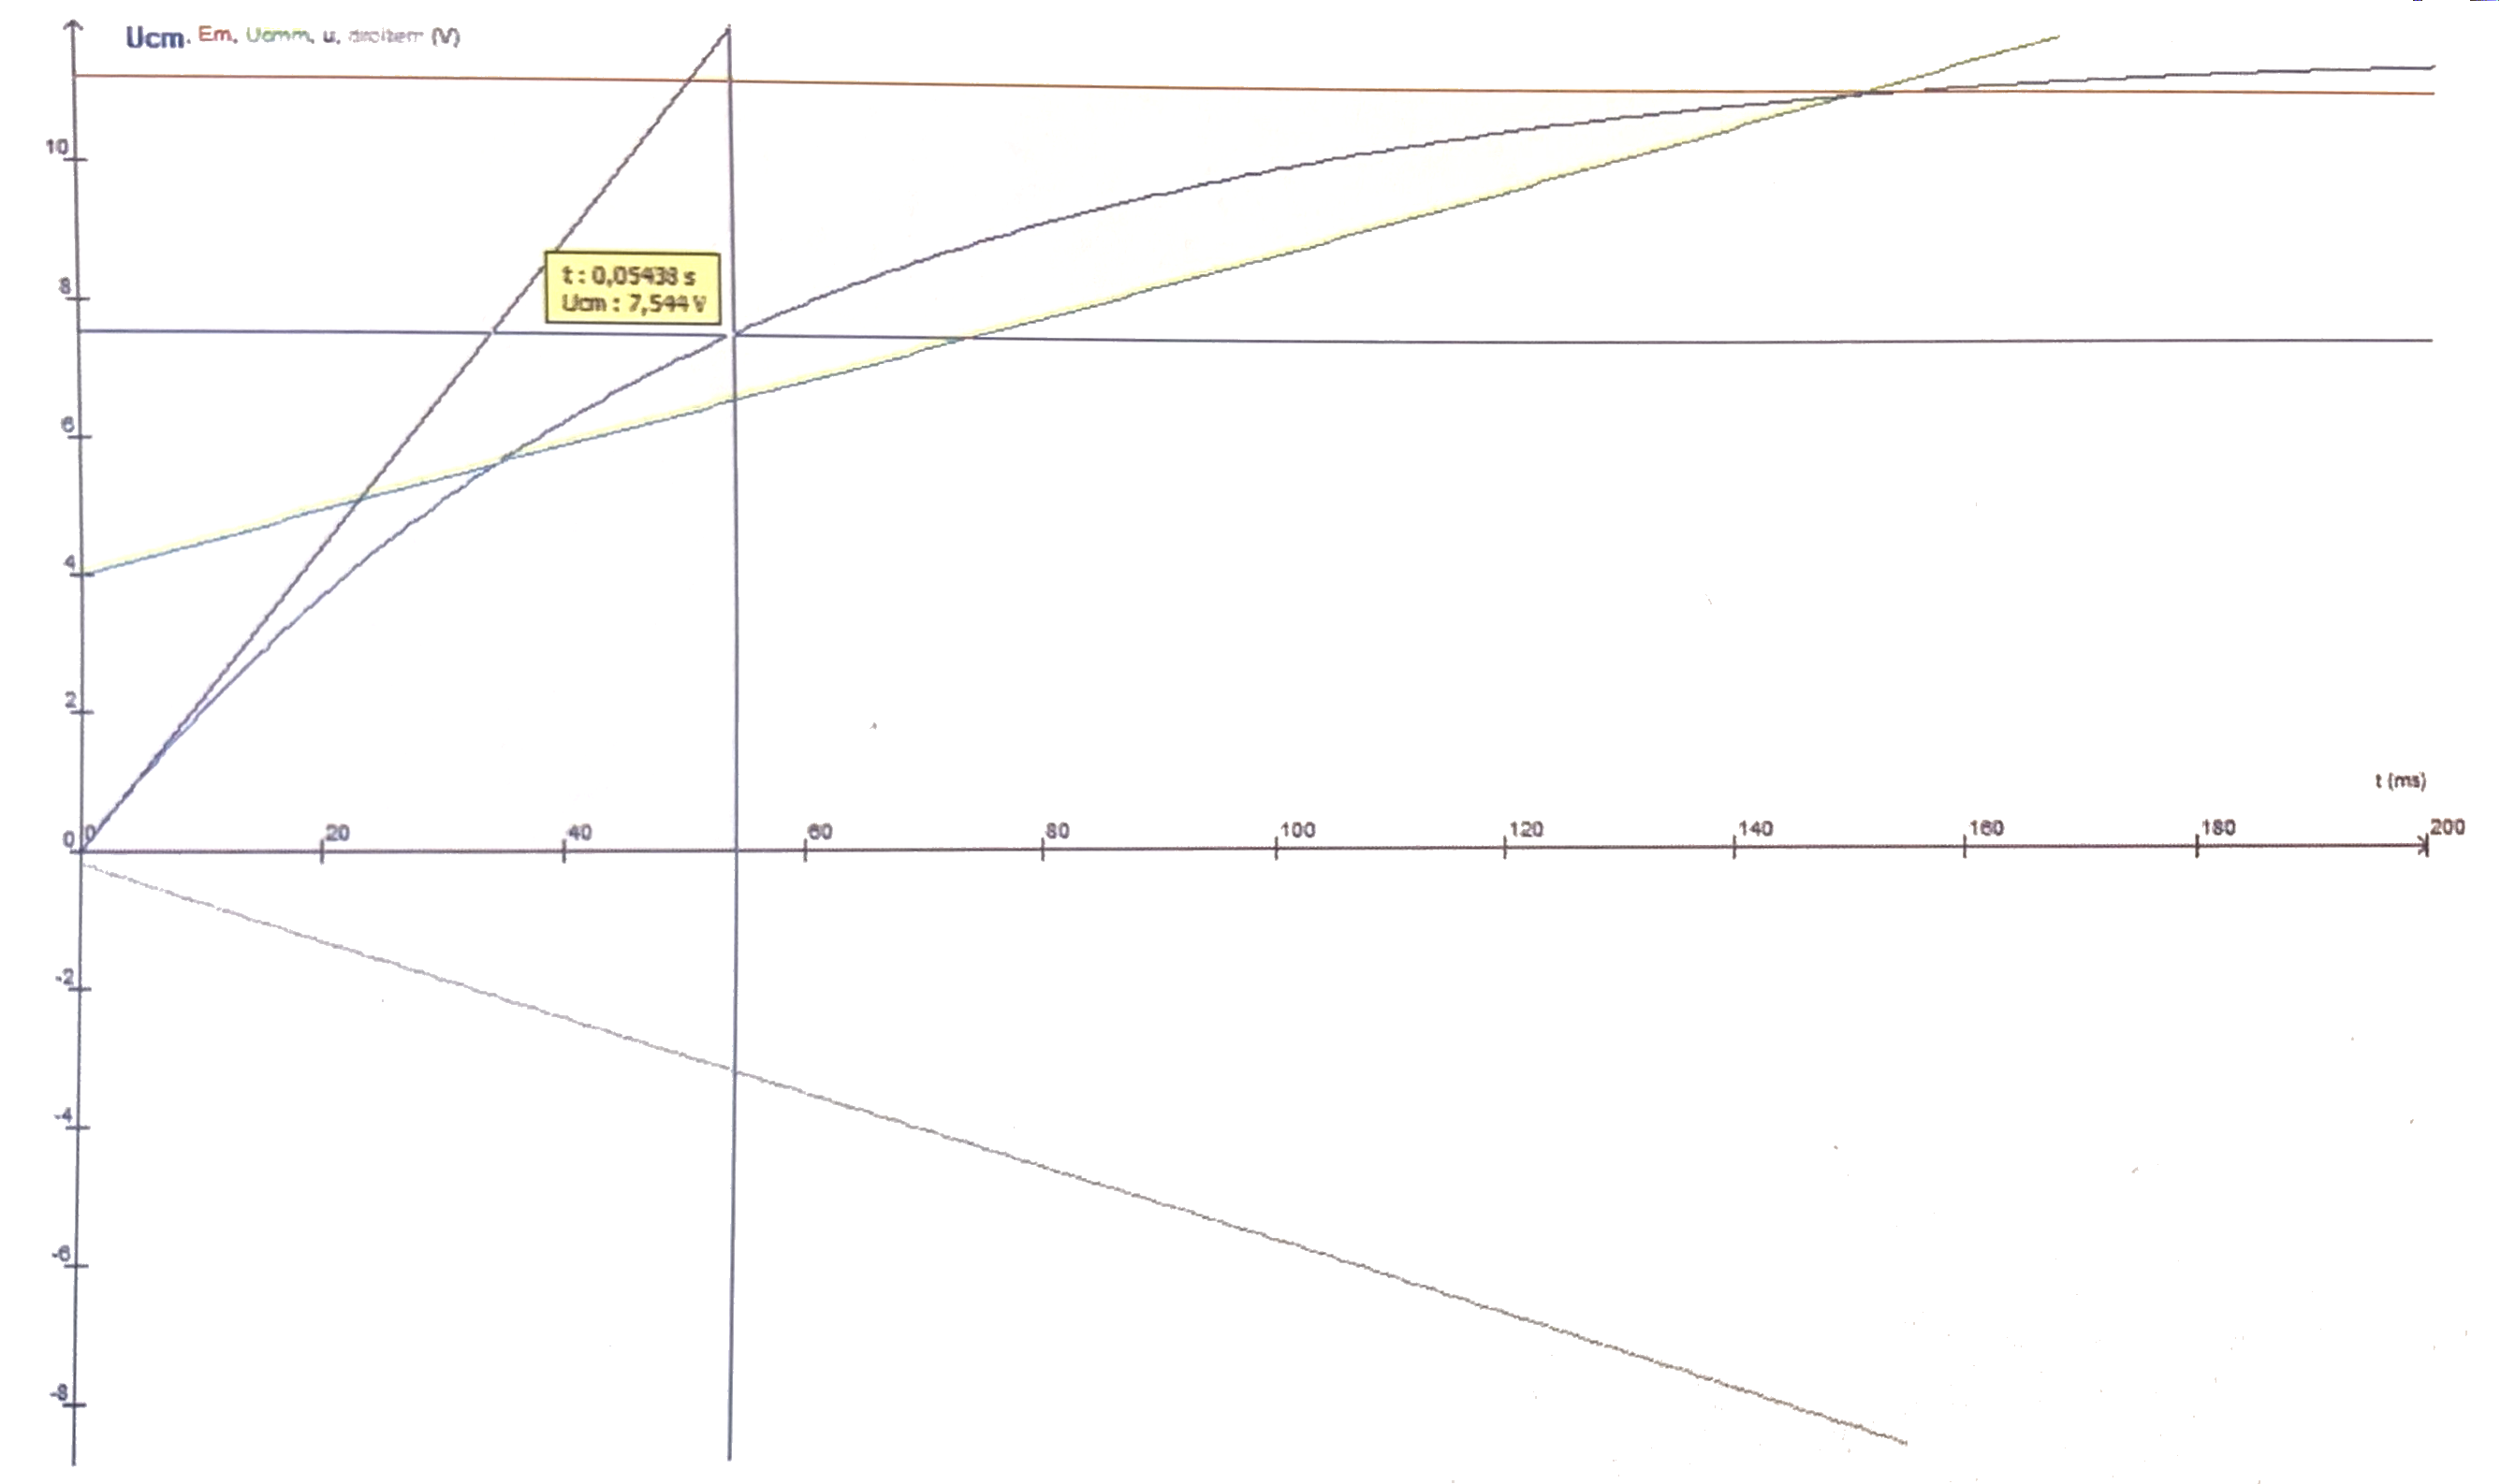
\includegraphics[width = 12cm]{graph.png}
\end{center}

\end{document}
